\chapter{Un poco sobre matroides}

\section{Un poco de independencia lineal}
Sea $V$ un espacio vectorial finito y sea $\mathcal{F}$ una colección de subconjuntos de $V$ con la propiedad que si $A$ pertenece a $\mathcal{F}$ es porque $A$ linealmente independiente. Cualquier persona que ha cursado un curso en álgebra lineal puede ver que se cumplen las siguientes tres cosas: 
    \begin{enumerate}
        \item El conjunto vacío ($\emptyset$) pertenece a $\mathcal{F}$.
        \item Si $X$ pertenece a $\mathcal{F}$ y $Y$ es un subconjunto de $X$, entonces $Y$ pertenece a $\mathcal{F}$.
        \item Si $X$ y $Y$ pertenecen a $\mathcal{F}$ y la cardinalidad de $X$ es 1 más la cardinalidad de $Y$, entonces existe un elemento $v$ en $X \setminus Y$ tal que $Y \cup \{v\} $ pertenece a $\mathcal{F}$. 
    \end{enumerate}
A partir de estos tres puntos podemos redefinir algunos conceptos básicos que se ven en álgebra lineal de una forma distinta pero equivalente. Definimos una \textbf{base} como un subconjunto de $V$ en $\mathcal{F}$ de cardinalidad máxima. Definimos el \textbf{rango} de un conjunto $A$ en $V$ como la cardinalidad del subconjunto de $A$ en $\mathcal{F}$ de mayor tamaño. 

\section*{Un poco de gráficas}
Sea $G = (V,E)$\footnote{Si el lector no tiene conocimientos de teoría de gráficas, recomendamos primero leer \cite{Mariana-Alice} que se encuentra en esta misma edición unas paginas adelante.} una gráfica %>,
definimos un \textbf{ciclo} como un camino cuyo origen y destino son el mismo vértice. Sea $\mathcal{F}$ una colección de subconjuntos de aristas ($E$) con la propiedad de que si $A$ pertenece a $\mathcal{F}$ es porque las aristas en $A$ no forman ningún ciclo. Vemos que esta familia de subconjuntos $\mathcal{F}$ también cumple las propiedades 1,2 y 3 de arriba \footnote{La demostración de esto es un poco larga, si el lector desea verla puede consultar \cite{ciclos}. }. Ahora, si definimos un \textbf{conjunto dependiente} como cualquier conjunto $A$ que no pertenece a $\mathcal{F}$ podemos redefinir a un ciclo como un conjunto dependiente minimal, esto es % >:
no existe $x$ en $A$ de tal forma que $A \setminus \{ x \}$ sea dependiente. 

\section*{Un poco de matroides}

Ahora, si dado un conjunto $S$ finito existe $\mathcal{F}$ tal que cumple con las propiedades 1,2 y 3 % >.
decimos que $(S,\mathcal{F})$ es una \textbf{matroide}. A esta colección de subconjuntos se le puede atribuir los conceptos de base, rango y ciclo mencionados anteriormente. Adicional a esto, definimos un \textbf{conjunto cerrado} como un conjunto $A$ con la propiedad de que su rango es menor estricto al rango de $A \cup \{ x \}$ para toda $x$ en $S \setminus A$. \\

Un par de conceptos que vale la pena mencionar son el de \textbf{lazo} y el de \textbf{paralelo}. Un lazo es una arista que empieza y acaba en el mismo vértice, desde el punto de vista de matroides es un elemento que por si solo es dependiente a pesar de ``no depender de nada" y en el caso de espacios vectoriales el cero es un lazo.  Se dice que dos elementos son paralelos si el conjunto que los contiene a ambos es dependiente, esto concepto en gráficas puede ser visto como dos aristas opuestas (una va de $a$ a $b$ y la otra de $b$ a $a$). 

\begin{figure}[h]\centering

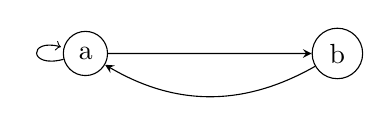
\begin{tikzpicture}[ scale=0.8]
\tikzset{vertex/.style = {shape=circle,draw,minimum size=1.5em}}
\tikzset{edge/.style = {->,> = latex}}

\node[vertex] (a) at (0,4) {a};
\node[vertex] (b) at (4,4) {b};


\path[-stealth] (a) edge (b);
\path[-stealth, bend left] (b) edge (a);

\path[-stealth,loop left] (a) edge (a);

\end{tikzpicture}

\caption{Una gráfica con dos aristas paralelas y un lazo.}
\end{figure}